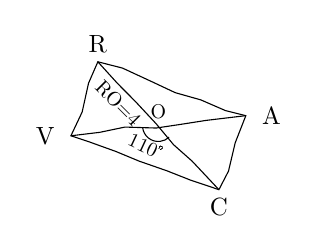
\begin{tikzpicture}[rotate=-20,every node/.style={scale=0.9},scale=1]

\coordinate (V) at (0,0);
\coordinate (R) at (0,1);
\coordinate (A) at (2,1);
\coordinate (C) at (2,0);
\coordinate (O) at (1,0.5);

\draw[decorate,decoration={random steps,amplitude=1pt,segment length=10pt}] (V) node [left=3pt]{V}--(R) node [above]{R}--(A) node [right=3pt] {A}--(C) node [below] {C}--cycle;
\draw [decorate,decoration={random steps,amplitude=1pt,segment length=10pt}] (V)--(A) (R)--(C);

\path (R)--(O) node[midway,below,rotate=-45,scale=0.8]{RO=4};
\node[above,scale=0.8] at (O){O};

\draw (0.82,0.41) arc (-153.43:-26.56:0.2) node[below=8pt,left,scale=0.8,rotate=-25]{110°};

\end{tikzpicture}